%\begin{frame}{What is Dynare?}
%	\begin{wideitemize}
%	    \item A free software platform for handling a wide class of economic models, in particular, DSGE models: Dynare is a collection of Matlab routines.
%	    \item Dynare is very user-friendly and has low entry costs
%	    \item Users provide a \texttt{.mod} file containing parameters, model equations linking the variables, and a list of computing tasks to be performed.
%	    \item Provides many state-of-the-art algorithms to handle DSGE models
%	    \item \url{https://www.dynare.org/} See also the Dynare manual\footcite{adjemian2022dynare}, the forum \url{https://forum.dynare.org/} and other resources e.g. \href{https://drive.google.com/file/d/1DO1OK5AKLWfcJX49ZPCGo58Ni2LdERw4/view}{An Introduction to Graphs in Dynare}
%	\end{wideitemize}
%\end{frame}
%
%\begin{frame}{Tools available in Dynare}
%	\begin{wideitemize}
%	    \item Compute solutions to an approximation of stochastic models, including models with OBCs
%	    \item Compute solutions to deterministic models, including models with OBCs
%	    \item Model estimations via Bayesian techniques or maximum likelihood, including models with OBCs
%	    \item Solve for optimal policy...
%	    \item ...and many more
%	\end{wideitemize}
%\end{frame}
%
%\begin{frame}{How Dynare works}
%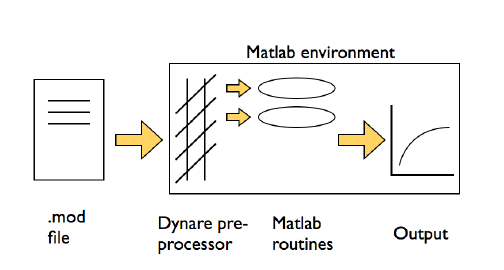
\includegraphics[width=0.8\textwidth]{figures/Dynare.PNG}\\
%\footnotesize{Source: Griffoli}
%\end{frame}


%\begin{frame}{A Dynare file}
%Our model:
%\begin{itemize}
%    \item Endogenous variables: $\pi_t, y_t, i_t, \varepsilon_t^a, \varepsilon_t^c, \varepsilon_t^i $
%    \item Some parameters: $ \beta, \kappa, \sigma,\phi_\pi,\phi_y,\rho^a, \rho^c, \rho^i $
%    \item Exogenous variables (shocks): $,u_t^a,u_t^c,u_t^i$ (see in the next slides)
%    \item Model equations
%    \begin{align*}
%        \pi_t =& \beta E_t\left[\pi_{t+1}\right]+\kappa y_t +\varepsilon_t^a \\
%        y_t =& E_t \left[y_{t+1} \right]- \frac{1}{\sigma}\left(i_t-E_t\left[\pi_{t+1}\right]\right)+\varepsilon_t^c \\
%        i_t =& \phi_\pi \pi_t + \phi_y y_t+\varepsilon_t^i
%        ...
%    \end{align*}
%\end{itemize}
%\end{frame}

%\begin{frame}{Structure of a Dynare file}
%\smartdiagramset{back arrow disabled,module minimum width=2.cm,font=\footnotesize}
%\smartdiagram[flow diagram:horizontal]{Preamble, Model definition, Steady state, Simulation and estimation}
%\begin{wideenumerate}
%\item Preamble: Declaration of endogenous and exogenous variables and parameters. Set value for calibrated parameters
%\item Model definition: State the dynamic model equations
%\item Steady state (long-run equilibrium)
%\item Additional computations: model checks,  simulation, estimation, ...
%\end{wideenumerate}
%\end{frame}

%\begin{frame}[fragile]{How to interact with Dynare: 1) Preamble}
%\begin{columns}
%\begin{column}[T]{0.5\textwidth}
%	    Our model:
%	    \begin{wideitemize}
%	        \item Endogenous variables: $\pi_t, y_t, i_t, \varepsilon_t^a, \varepsilon_t^c, \varepsilon_t^i$
%	        \item Exogenous variables (shocks): $u_t^a, u_t^c, u_t^i$
%	        \item Parameters: $ \beta, \kappa, \sigma,\phi_\pi,\phi_y,\rho^a,\rho^c,\rho^i $
%	    \end{wideitemize}
%\end{column}
%\begin{column}[T]{0.5\textwidth}
%Dynare code
%\begin{minted}{c++}
%var // endo vars
%pie y inom zeps_a zeps_c zeps_i;
%
%varexo
%u_a u_c u_i;
%
%parameters
%betta kappa sig phi_pi
%phi_y rho_a rho_c rho_i;
%\end{minted}
%\end{column}
%\end{columns}
%\end{frame}
%
%\begin{frame}[fragile]{How to interact with Dynare: 1) Preamble (cont'd)}
%\begin{columns}
%\begin{column}[T]{0.5\textwidth}
%	    \begin{wideitemize}
%	        \item Set $\beta$ and $\kappa$ to conventional values informed by real interest rates and price adjustment frequencies
%	        \item Choose parameters for the Taylor rule
%	        \item Set autocorrelation coefficients
%	        \item Unit intertemporal elasticity of substitution
%	    \end{wideitemize}
%\end{column}
%\begin{column}[T]{0.5\textwidth}
%\begin{minted}{c++}
%// Calibration
%betta   = 0.99;
%phi_pi  = 1.5;
%phi_y   = 0.2;
%kappa   = 0.12;
%rho_a   = 0.8;
%rho_c   = 0.8;
%rho_i   = 0.5;
%sig     = 1;
%\end{minted}
%\end{column}
%\end{columns}
%\end{frame}
%
\begin{frame}[fragile]{Dynare code: Core part of the model}
%\begin{columns}
%\begin{column}[T]{0.5\textwidth}
%	    \begin{wideitemize}
%	        \item Dynare allows writing the model in a very natural way
%	        \item Keyword \texttt{model;} indicates begin of model declaration. The argument \texttt{linear} instructs Dynare that our model is already linearised (the software can do it for you too)
%	        \item \texttt{(+1)} indicates expected (one-period ahead) variables. No expectations operator needed.
%	        \item \texttt{(-1)} indicates lagged variables
%	    \end{wideitemize}
%\end{column}
%\begin{column}[T]{0.5\textwidth}
\begin{minted}{c++}
model(linear);
[name='Phillips Curve']
pie=betta*pie(+1)+kappa*y+zeps_a;

[name='IS curve']
y=y(+1)-1/sig*(inom-pie(+1))+zeps_c;

[name='Notional rate Taylor rule']
inomnot=rhoinom*inomnot(-1)
        +(1-rhoinom)*(phi_pi*pie+phi_y*y)+zeps_i;
\end{minted}
%\end{column}
%\end{columns}
\end{frame}


%\begin{frame}[fragile]{Timing conventions}
%\begin{wideitemize}
%    \item A variable decided at time $t$ enters as a contemporaneous variable.
%    \item Predetermined variables enter as $t-1$, i.e. \texttt{X(-1)}.
%    \item For example, in the typical RBC model, the capital stock used in period $t$ is decided in $t-1$.
%    \begin{itemize}
%        \item The law of motion in this convention follows $K_t = (1-\delta)K_{t-1}+I_t$.
%    \end{itemize}
%    \item Keyword \href{https://www.dynare.org/manual/the-model-file.html?highlight=predetermined#predetermined_variables}{\texttt{predetermined\_variables}} changes the convention.
%    \item Shocks occur at the beginning of the period.
%\end{wideitemize}
%\end{frame}
%
%\begin{frame}[fragile]{Timing conventions: Code}
%\begin{columns}
%\begin{column}[T]{0.5\textwidth}
%Example using the default convention (see reference manual)
%\begin{minted}{c++}
%var y, k, i;
%...
%...
%model;
%y = k(-1)^alpha;
%k = i + (1-delta)*k(-1);
%...
%end;
%\end{minted}
%\end{column}
%\begin{column}[T]{0.5\textwidth}
%Example using the  \href{https://www.dynare.org/manual/the-model-file.html?highlight=predetermined#predetermined_variables}{\texttt{predetermined\_variables}} command:
%\begin{minted}{c++}
%var y, k, i;
%predetermined_variables k;
%...
%model;
%y = k^alpha;
%k(+1) = i + (1-delta)*k;
%...
%end;
%\end{minted}
%\end{column}
%\end{columns}
%\end{frame}
%
%\begin{frame}[fragile]{How to interact with Dynare: 3) Steady state}
%\begin{columns}
%\begin{column}[T]{0.5\textwidth}
%	    \begin{wideitemize}
%	        \item Our model is expressed in deviation from the steady state (around zero inflation).
%	        \item Thus, all variables are zero in the steady state.
%	        \item The deterministic steady state implies no shocks: $u= 0.$
%	        \item All shock processes are 0 too: $\bar{\varepsilon} = \rho \bar{\varepsilon} +0 \longrightarrow \bar{\varepsilon} = 0.$
%	        \item Check with \href{https://www.dynare.org/manual/the-model-file.html?highlight=steady#steady}{\texttt{steady;}}-command
%	    \end{wideitemize}
%\end{column}
%\begin{column}[T]{0.5\textwidth}
%\begin{minted}{c++}
%steady_state_model;
%pie=0;
%y=0;
%inom=0;
%zeps_a=0;
%zeps_c=0;
%zeps_i=0;
%end;
%steady;
%\end{minted}
%\end{column}
%\end{columns}
%\end{frame}
%
%
%\begin{frame}[fragile]{Steady state}
%\begin{wideitemize}
%    \item Dynare can solve for the steady state using initial starting values provided.
%\begin{minted}{c++}
%initval;
%y=0;
%end;
%\end{minted}
%    \item Inside \texttt{steady\_state\_model;} you can define variables recursively and use auxiliary definitions.
%    \item Always use a fully analytical steady state if possible (especially for estimations!)
%    \item The steady state values stored in \texttt{oo\_.steady state} follow the declaration order.
%    \item You can also calculate the steady state using your own numerical routines.
%    \begin{itemize}
%        \item Create a Matlab file with the same name as your model followed by \texttt{\_steadystate}.
%        \item For example,  \texttt{DSGE\_steadystate.m} for model file \texttt{DSGE.mod}
%    \end{itemize}
%\end{wideitemize}
%\end{frame}
%
%\begin{frame}[fragile]{Steady state m-file}
%\begin{minted}{matlab}
%function [ys check] = dsge_steadystate(ys,exo)
%global betta
%rss = 1/betta;
%ys=[rss];
%check=0;
%\end{minted}
%\begin{itemize}
%    \item Alphabetical output
%    \item You can use function solvers here.
%    \item Full example available \href{https://github.com/DynareTeam/dynare/blob/master/examples/NK_baseline_steadystate.m}{here [LINK].}
%\end{itemize}
%\end{frame}
%
%
%
%\begin{frame}[fragile]{Composite parameters}
%\begin{wideitemize}
%    \item Sometimes, parameters are functions of other parameters.
%    \item They can be calibrated in the \texttt{steady\_state\_model}-block.
%    \item Or, alternatively, in the \texttt{model} block, using the \# operator.
%\begin{minted}{c++}
%model(linear);
%#kappa = (sig+eta)*(1-theta)*(1-betta*theta)/theta;
%
%pie=betta*pie(+1)+kappa*y+zeps_a;
%\end{minted}
%    \item Accounting for these dependencies is important - especially for estimation. Why?
%\end{wideitemize}
%\end{frame}


%\begin{frame}[fragile]{Macro processor}
%\begin{wideitemize}
%\item For larger models and modular code, the Dynare macro processor is helpful.
%\item See \url{https://www.dynare.org/assets/team-presentations/macroprocessor.pdf} for many examples.
%\begin{itemize}
%\item Allows for \texttt{if} and \texttt{for} loops.
%\begin{minted}{c++}
%@#define occbin = 0
%@#if occbin
%    occbin_setup;
%@#endif
%\end{minted}
%\item Include more files:
%\begin{minted}{c++}
%@#include "observation_equations.inc"
%\end{minted}
%\end{itemize}
%\end{wideitemize}
%\end{frame}

%\begin{frame}[fragile]{Running Dynare}
%\begin{wideitemize}
%    \item You need to add Dynare to your Matlab path, e.g.
%    \begin{minted}{matlab}
%    addpath c:/dynare/x.y/matlab
%    \end{minted}
%    \item You can run the model file and invoke Dynare using
%    \begin{minted}{matlab}
%    dynare FILENAME[.mod]
%    \end{minted}
%    \item Dynare stores results, model information, and selected options in Matlab structures (use the tab key to access the different fields)
%    \begin{itemize}
%        \item \texttt{oo\_} stores results from computations (simulation results, ...)
%        \item \texttt{M\_} stores model information (e.g. info on parameters and their values)
%        \item \texttt{options\_} stores the selected options.
%    \end{itemize}
%\end{wideitemize}
%\end{frame}
%
%\begin{frame}[fragile]{How to interact with Dynare}
%\begin{wideitemize}
%\item You can integrate Dynare into Matlab files
%\begin{itemize}
%    \item Be careful as Dynare clears the memory. You can avoid this using the option \texttt{noclearall}
%    \begin{minted}{matlab}
%    dynare example.mod noclearall
%    \end{minted}
%
%\end{itemize}
%    \item Let me show you a concrete model code.
%    \item After that, before discussing specific simulation commands, let's review what Dynare is doing behind the scenes.
%\end{wideitemize}
%\end{frame} 